\chapter{Introduction}
\label{chap:introduction}

\section{Motivation}
Current Blimp technology relies on a design that is self stable in a desired orientation, thus enabling very simple control.
This limits the movement of the blimp to very slow speeds and also makes them appear clumsy.
Especially eye-catching are specifically shaped blimps, e.g. blimps that have the shape of a mascot, car or any other commercial product (see figure \ref{fig:blimps}).
%As an alternative, conventionally shaped blimps can show imprints or banners.
The arrangement of the actuators for those different shaped blimps varies a lot.
In general, manual adjustment of the control algorithms is needed or the actuators have to be controlled manually.
Our idea is to use some adequate sensors to determine the effect of the actuator on the movement of the blimp.
When such an algorithm is available, the blimp hull can be manufactured independently on the actuation units which can then be attached to the blimp.
The actuators' effect on the system is then automatically detected by the identification algorithm and this knowledge is used to control the system.
This is illustrated by \cref{fig:motivation}.

\begin{figure}[hbtp]
\centering
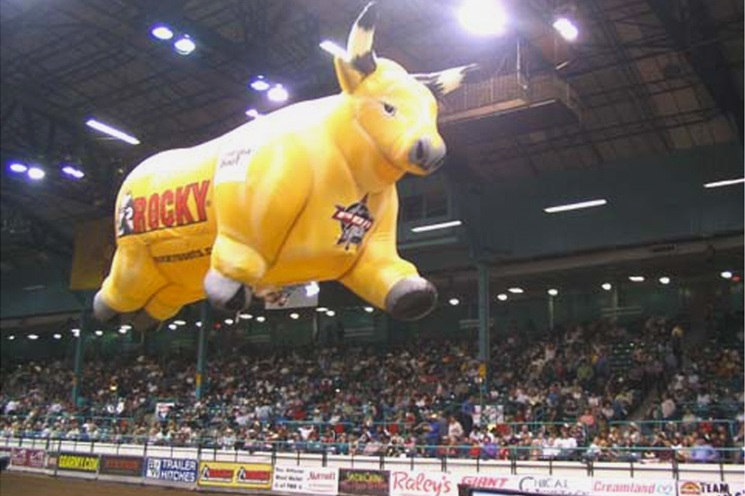
\includegraphics[width=.45\linewidth]{images/intro/CustomBull_Lg.jpg}
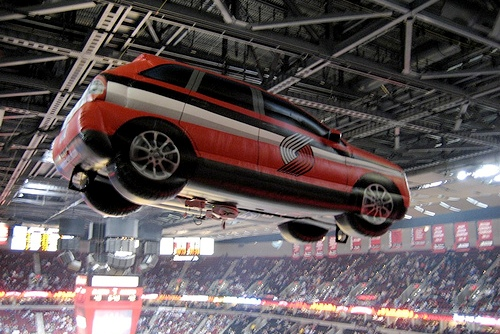
\includegraphics[width=.45\linewidth]{images/intro/CustomCar.jpg}
\caption{Custom shaped blimps are used for advertising \citep{rcblimps}.}
\label{fig:blimps}
\end{figure}

\begin{figure}[hbtp]
\centering
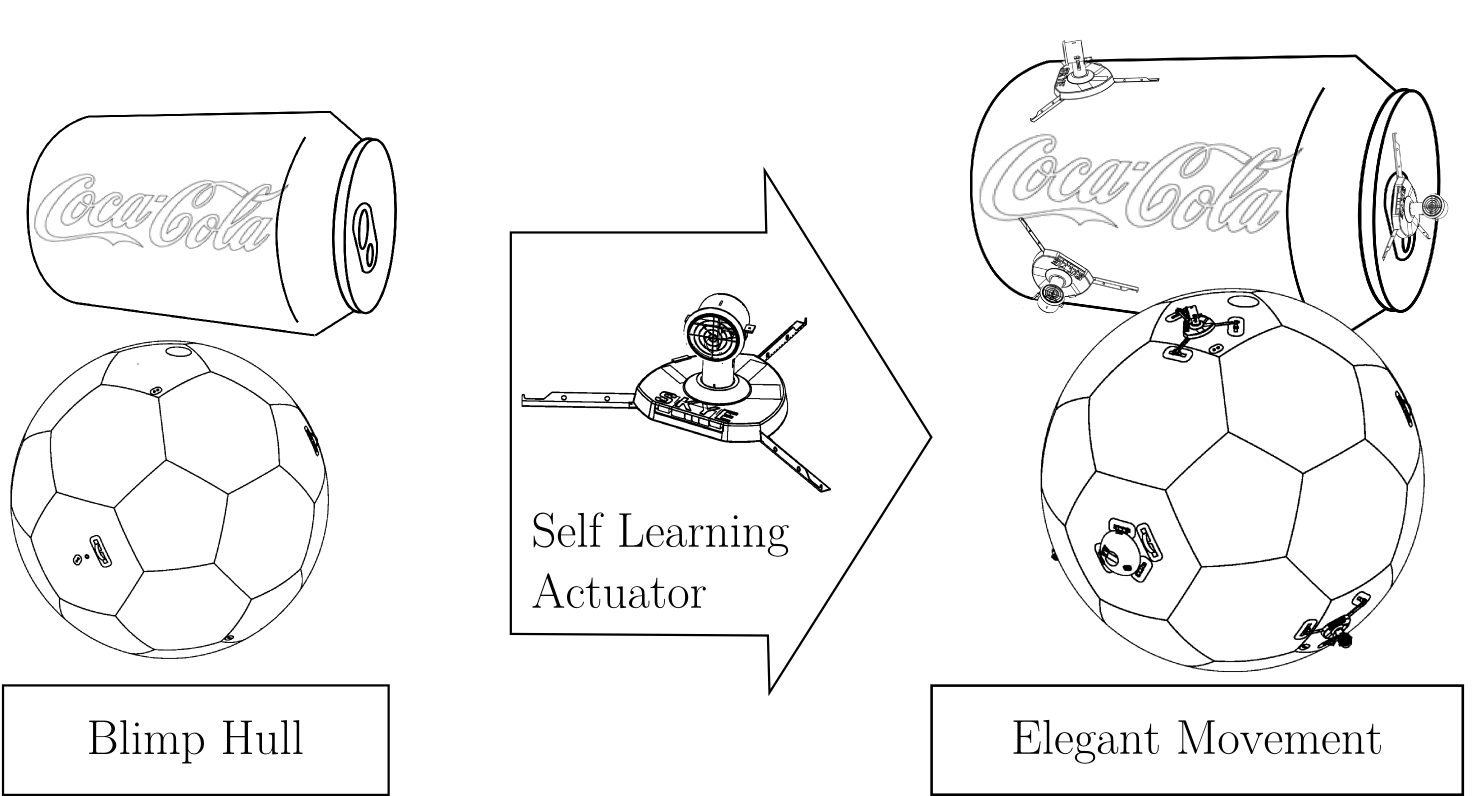
\includegraphics[width=.85\linewidth]{images/intro/motivation.png}
\caption{The goal is to find an algorithm, that allows to take any blimp hull (\textbf{left}) and attach the actuation units (\textbf{center}).
The actuation configuration is then automatically detected, such that elegant movements can be performed without manual controller adjustments (\textbf{right}).}
\label{fig:motivation}
\end{figure}

\section{Related Work}
\label{sec:rel_work}
This thesis is on estimation of the actuation configuration for a multi-actuated blimp. \\
Various work on thruster configuration estimation can be found for underwater robot systems.
\Citet{Doniec} propose black-box model approach.
They calculate an inverse model of the thrusters, i.e. a mapping from a desired rotation and position change of the robot to the thruster commands. After about 40 seconds of random walk, the inverse model is computed as the Moore-Penrose pseudoinverse of the collected input/output data.
\Citet{VandeVen2005} show an overview of neural network control of underwater vehicles. \\ 
If a first principle-based model of the system is available, gray-box modelling may be applied.
Many aerospace and robotics tasks are solved using physical meaningful models.
To determine the sensor alignments after launch shock, \citet{Shuster1991} estimate the rotation vector between multiple star tracker devices using batch optimization.
\Citet{Bloesch2013} formulated a nonlinear least squares problem to estimate kinematic parameters of a legged robot.
In depth studies using batch optimization have been made for intrinsic and extrinsic (stereo) camera calibration \citep[chap. 4]{Siegwart}.
In recent time, visual-inertia sensor calibration has found much attraction.
Beside others, \citet{Hol2011} showed both batch and recursive estimation (Kalman Filter) for this task.

\section{Skye System Overview}
The experimental part of this thesis is done with the Skye System \citep{Skye2013}.\\
Skye is a spherical blimp (\cref{fig:frames}, right) where the center of gravity (COG) coincides with the center of buoyancy (COB).
Four identical actuators (\cref{fig:frames}, left) are attached to the hull of Skye in a tetrahedral arrangement.
Each of those actuator units consists of a static platform and part that can be rotated around the vertical axis.
Mounted to the rotating part of the actuators there is an impeller which can generate thrust.
% in the XY-plane along the direction it is currently pointed.
This setup gives Skye the ability to move and rotate in all directions with more or less the same efficiency \citep[see][chap. 3]{Schaffner2012}.

\subsection{Coordinate Systems}
\label{sub:coordinate_systems}
Different coordinate systems are used in this thesis to represent the blimp states and the actuation properties (see \cref{fig:frames}).
\begin{description}
\item[The world frame ($w$-frame)] is a stationary North-East-Down (NED) frame (\cref{fig:frames}, bottom).
\item[The blimp frame ($b$-frame)] is a blimp body fixed frame (\cref{fig:frames}, right).
When the camera is upright and pointing north, it matches a north-east-down (NED) frame.
Its origin coincides with the center of gravity of the blimp.
\item[The motor frames ($m^k$-frame)] (\cref{fig:frames}, left) are aligned to each actuator units $k=1,...,N$.
When the actuator is placed on a horizontal surface, $\mathbf{e}_{m^k}^z$ is defined to point downwards.
The coordinate system origin is set to the base of the actuator such that the z-axis coincides with the rotation axe of the actuator.
$\mathbf{e}_{m^k}^x$ is defined to be pointing in the direction of the thruster when its orientation angle $\alpha^k$ is zero (see \cref{fig:motor_force}).
%To put it another way, the thrust-force points in the x-axis direction when the actuator angle is zero.
\item[The tangential reference frames ($t^k$-frame)] are used to express the estimated actuator configuration.
If the true position and orientation of the motors is known (e.g. in simulation), $t^k$ is the coordinate frame for the true motor position and orientation, whereas $m^k$ is the frame for the estimated ones.
If the true position is not known (e.g. for real data), any close estimate to the true is taken for $t^k$ and serves as a common frame to compare multiple estimates.
The use for this frame will become clear in \cref{sec:comparing_results}.
\end{description}

\begin{figure}[hbtp]
\centering
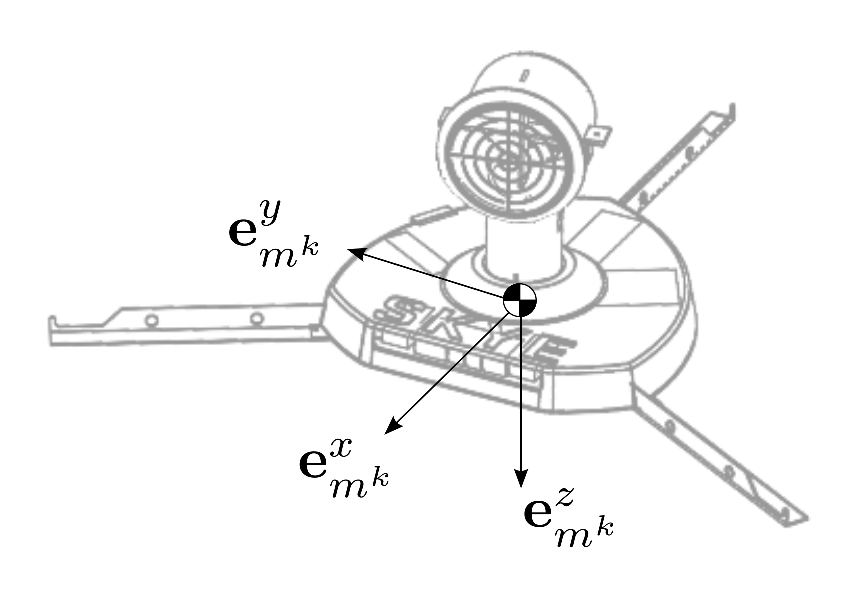
\includegraphics[scale=.4]{images/intro/motor_frame.eps}
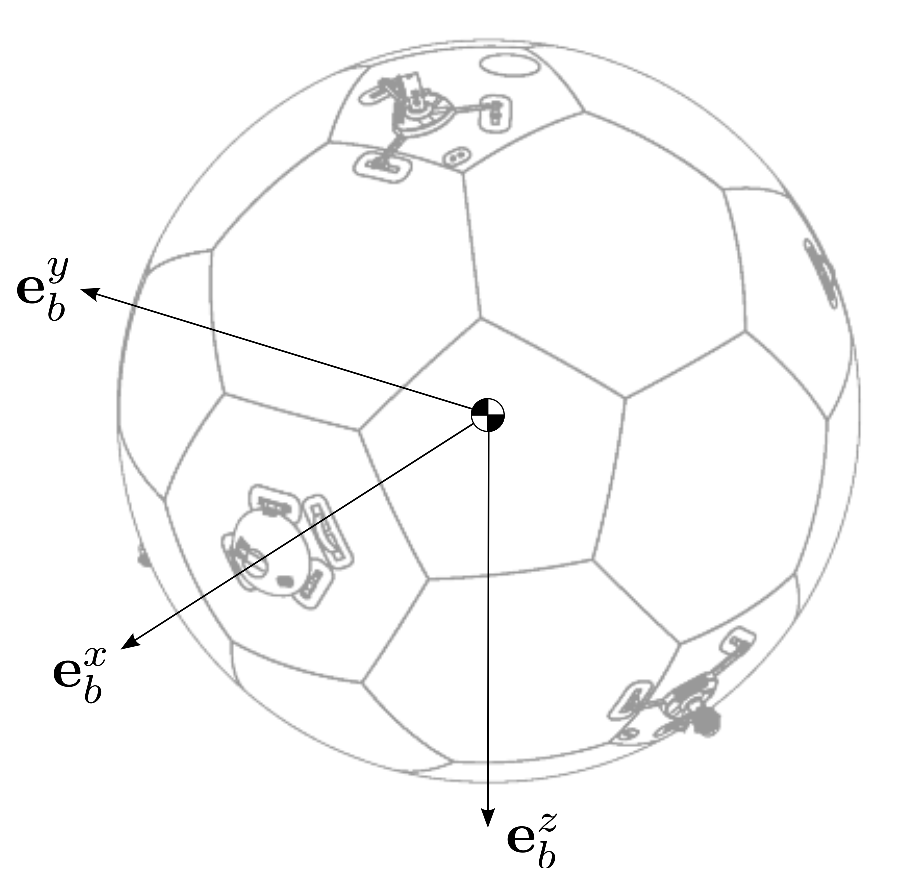
\includegraphics[scale=.4]{images/intro/blimp_frame.eps} \\
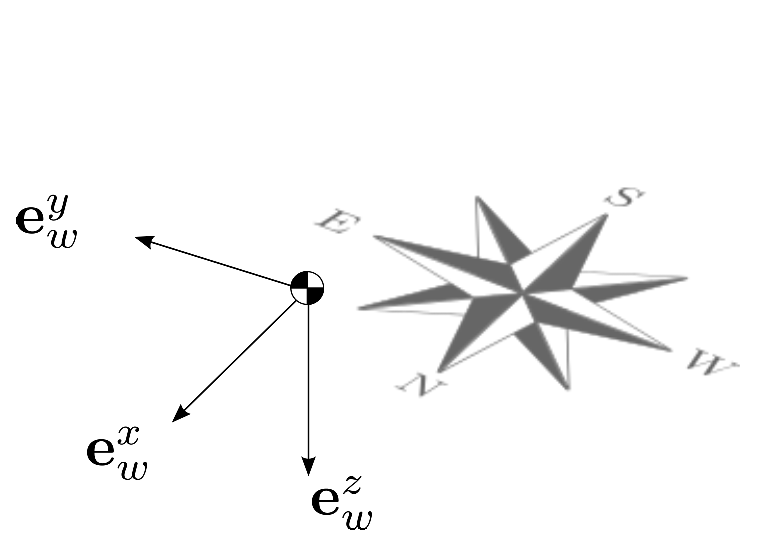
\includegraphics[scale=.4]{images/intro/world_frame.eps}
\caption{\textbf{Left}: Motor coordinate frame $m^k$. When the thruster is not rotated, it directs in $\mathbf{e}^x_{m^k}$ direction. $\mathbf{e}^z_{m^k}$ directs to the bottom.
\textbf{Right}: Blimp coordinate frame $b$. $\mathbf{e}^x_{b}$ directs to the camera which is mounted at the front. 
$\mathbf{e}^z_{b}$ directs to the bottom.}
\label{fig:frames}
\end{figure}

Now as we have introduced the coordinate systems, we can formulate the force vector $\mathbf{F_{m^k}^k}$ generated by the actuation unit $k$ expressed in its local motor frame $m^k$ as
\begin{equation}
\mathbf{F_{m^k}^k} = 
\left[\begin{array}{c}
F^k \cos(\alpha^k) \\
F^k \sin(\alpha^k) \\
0
\end{array}\right]
\end{equation}
as it is shown in \cref{fig:motor_force}.
$\alpha^k$ is the orientation angle around $\mathbf{e}_{m^k}^z$ and $F^k$ is the thrust force magnitude.

\begin{figure}[hbtp]
\centering
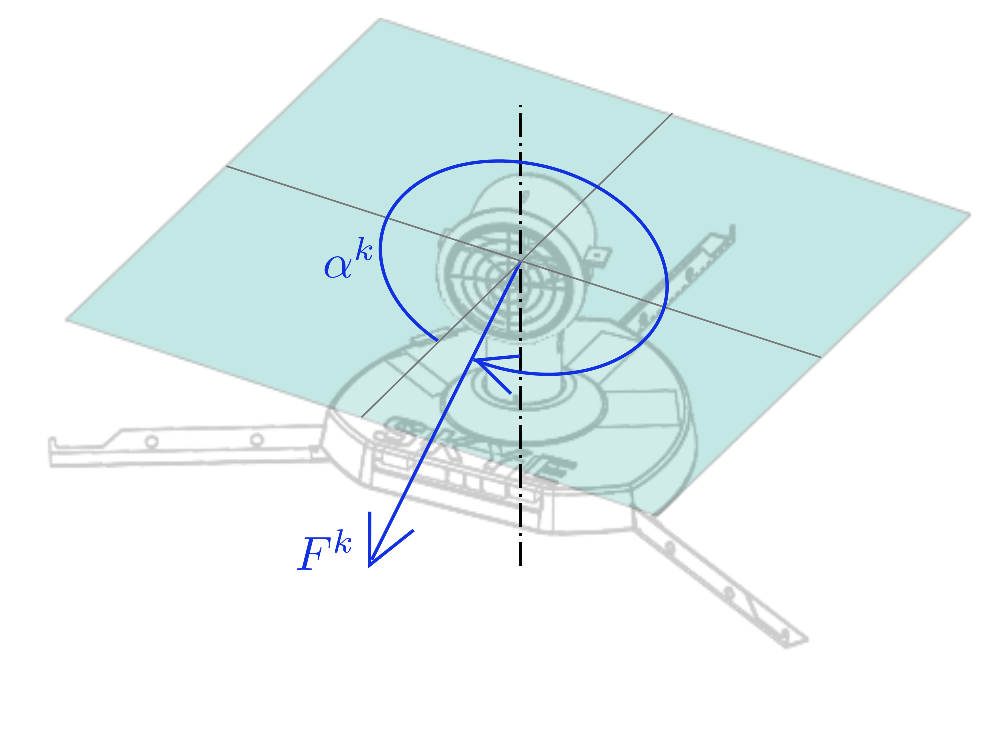
\includegraphics[width=.4\linewidth]{images/intro/motor_force.eps}
\caption{Motor orientation angle $\alpha^k$ and thrust force $F^k$.}
\label{fig:motor_force}
\end{figure}

\subsection{Hardware and Software}
The control hardware and software of Skye is based upon the framework from the \textsc{Pixhawk} Research Project \citep{pixhawk}.
The firmware of Skye is based on \textsc{Pixhawk}'s PX4FMU device which includes an IMU.
For operating Skye, a \textsc{QGroundControl} based interface is installed on a laptop
which is connected via a \textsc{XBee} link to the PX4 autopilot.
Piloting is possible by a 3D mouse from \textsc{3DConnexion} \citep[see][]{Krebs2012}.

\subsection{Sensors}
The sensors used for this thesis are part of the PX4FMU.
Although there are some more sensors on the device, the most relevant sensor is the MPU-6000 Six-Axis (Gyro + Accelerometer) MEMS MotionTracking™ Device.
This sensor measures angular velocities around three axes as well as translational acceleration in three directions. \\
To get an understanding of the performance of the gyro of the MPU-6000, we measured the noise to be about $3.2 \cdot 10^{-4}rad/s$ RMS (see Appendix \cref{fig:gyro_noise}).

\subsection{Allocation}

\begin{figure}[hbtp]
\centering
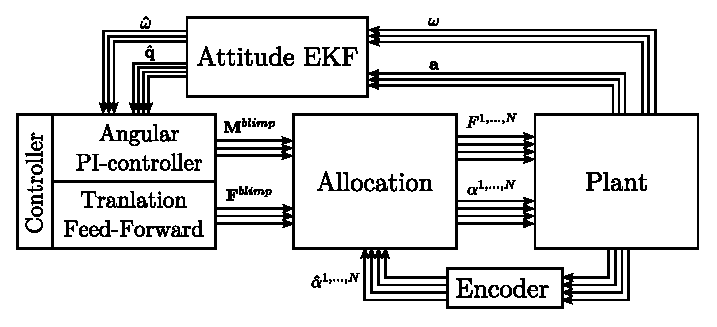
\includegraphics[width=.9\linewidth]{images/intro/system_loop.eps}
\caption{Skye control loop. The allocation transforms the blimp control force and moment to the actuator signals. Good knowledge about the actuator configuration is required to achieve precise control.}
\label{fig:system_loop_3}
\end{figure}

One characteristic feature of Skye is the way controlled flight is achieved. 
\Cref{fig:system_loop_3} shows the control loop of Skye.
Because the four actuators have 8DOF in total and the flying body has only 6DOF that are subject to control,
the mapping between the controller output and the actuator inputs is not unique.
This mapping is designed to use minimal power consumption.
This is solved as a constraint optimization problem.
An analytical solution for the linear mapping has been derived by \citet{Schaffner2012} using Lagrangian multipliers.
For the constraints of this optimization problem, it is crucial to know the position and orientation of the motors.
Because Skye is over \unit[2.5]{m} in diameter it is difficult to measure the actuation configuration precisely.
The current system uses the actuator position from CAD data of Skye.


\section{Problem Evaluation}
\label{sec:problem_evaluation}
The main goal of this thesis is the \textit{Estimation of Actuation Configuration for a Multi-Actuated Blimp}.
The need for a good estimate of the actuation configuration is mainly given by the allocation part of the controller as described before.
Additional value can be achieved by estimating further properties, e.g. the offset between COG and COB.
If this offset is known, it is possible to calculate the required taring weight apportionment to get any desired COG offset\footnote{
In the simulation (see \cref{sec:simulation}), such an algorithm is already implemented to place the taring weights.
}.

\paragraph{Optimization Method Selection} ~\\
As it becomes clear by reading related work in section~\ref{sec:rel_work}, there exist various methods for system calibration.
% DOES SYSTEM IDENTIFICATION INCLUDE ONLINE EXTIMATION?
In general, online estimation techniques are preferred for dynamically changing properties (state estimation).
Offline estimation is preferred for estimating constant properties (parameter estimation).
The actuation configuration is assumed to be constant over a significant period of the flight time.
Therefore we will use offline estimation in this thesis.
%Nevertheless, a combined (online) estimator for parameters and states would be interesting but goes beyond the scope of this thesis. (??chame de satz nöd wegloh??)
\\

Offline estimation means that we collect a batch of data and calculate the estimate of the actuation configuration out of this data.
If the parameters change slowly over time, it is also possible to repeat the batch optimization after some time to consider these changes.
\\

For the estimation of the actuation configurations, we assume the system states to be known.
We will use the available information about the states from the online state estimator which is already implemented on the system.

\paragraph{Restriction to Spherical Blimps} ~\\
For the experimental validation in this thesis, we will use the Skye System.
Since Skye is a spherical blimp we can only verify the algorithm for spherical systems.
Because of this, we decided to focus the limited scope of a semester thesis on just spherical blimps.
\\

However, we designed the framework such that it can be expanded for the estimation of arbitrary actuator positions.
Some aspects as observability need to be considered when expanding the optimization task.
The thoughts outlined in \cref{sub:observability} will serve as a useful base.

\paragraph{System Model Selection} ~\\
For bulky, but rotation symmetric systems as blimps, aerodynamic effects have much more influence on the translational movements than on the rotational movements.
Effects like flow separation, drag crisis or the inertia of the surrounding fluid mainly influence the translational movements.
On rotational movements, aerodynamic effects have a much smaller impact.
Since it is a difficult task to model aerodynamic effects and this would lead to many more unknown parameters, we decided to restrict ourselves on the investigation of the rotational movement.
%We will see below that this approach is greatly capable of estimating the actuation configuration on a spherical blimp.

%...Title is \textsc{Estimation of Actuation Configuration for a Multi-Actuated Blimp}
%...inside System Identification methods, why did we pick batch optimization
%...why did we restrict to Gyro / angular acceleration